\documentclass[11pt,a4paper]{article} 
\usepackage[danish]{babel}
\usepackage[utf8]{inputenc}
\usepackage{amsthm,amssymb,amsmath,dsfont,mathrsfs,nicefrac} 
\usepackage{graphicx}

\begin{document}


\section{Undersøgt problem}

Koncentrationen har som efter tidsplanen ligget på at undersøge shadow mapping algoritmen. Der er blevet undersøgt tre forskellige måder at lave shadow mapping på og disse er blevet sammenlignet og den ene metode er blevet valgt, teorien er beskrevet og implementering er igang. 

Det næste afsnit beskriver de tre shadowmapping metoder der er undersøgt.



\section{Forskellige shadow mapping metoder}

Dette afsnit vil undersøge nogle af de forskellige metoder at ligge skygge på en scene, der arbejder i billede opløsning. Tre af metoderne vil blive studeret og beskrevet. Fordele og ulemper opstilles og diskuteres, der vil herefter blive valgt en metode at gå i dybden med samt lave en implementering af denne. Metoderne som vil blive sammelignet er:

\begin{enumerate}
  \item Shadow mapping med Percentage Closer Filtering (PCF)
  \item Perspetive Shadow Mapping (PSM)
  \item Cascaded shadow maps (CSMs)
\end{enumerate}

Nr 1. er den "original" shadow mapping algoritme udgivet i 1987 \cite{SMAP}, rapporten vil dog kigge på algoritmen med Percentage Closer Filtering for løsning af aliasing problmer. Metode to og tre er modifikationen af nr. 1 disse modifikationen er lavet for at løse nogle af aliasing problemerne med shadow mapping algoritmen (Nr.1). De efterfølgende underafsnit vil kort forklare metoderne og herefter diskutere disse med henblik på at arbejde videre med den mest brug bare løsning.

\subsection{Shadow maps med PCF}

Shadow mapping \cite{SMAP} er en teknik der arbejder i billedopløsninger, ideen er at flytte kameratet op til lystkilden og tage et billede hvor kun dybderne gemmens(shadow mappet). Kameraet flyttes nu tilbage til øjet og for hver fragtment sammenlignes fragtmentes dybde med den sammen fragtment men projekteret over i shadow mappet, hvis dybden i shadow mappet er mindre er punktet i skygge fordi der er et punkt set fra kameraet der er nærmere. Da der kun arbejdes i billedopløsninger kan der opstå en del geometiske fejl samt over og undersamplings fejl der kan give fejlagtige skygger. Disse problemer kan tildels løses ved at bruge en bias og et filter kendt som Percentage Closer Filtering. Dette giver en tilfredsstillende algoritme.

Fordele
\begin{itemize}
  \item Hurtigt og egner sig godt til real-time grafik.
  \item Shadow mappet skal kun opdateres hvis lyset eller objekter flyttes ikke kameraet.
\end{itemize}

Ulemper:
\begin{itemize}
  \item Store aliasing problemer der dog tildels kan løses med PCF.
  \item Kræver scenen skal tegnes mindst to gange.
\end{itemize}


\subsection{Perspective Shadow maps}

Perspective Shadow Maps \cite{PSMAP} blev publiciteret i 2002 af Stamminger og Drettakis, denne metode bygger på videre på den originale shadow mapping ide \cite{SMAP}. Teknikken prøver at løse de alaising problemer der opstår i Shadow mapping, ved at justere den uniforme sampling fordeling i shadow mappet. Forbedring opnås ved at genere shadow mappet i \textit{Post-perspective Space} for kameraet, inden det perspective shadow map bliver generet bliver scenen og lyset transformeret med kamerates matrix. Dette betyder at objekter tæt på kameraet vil have en højere sampling, til forskel fra shadow mapping hvor samplingen factoren i forhold til objekter kun afhænger af deres placering i forhold til lyset og ikke kameraet.


Fordele
\begin{itemize}
  \item Løser i de fleste tilfælde aliasing problemer med shadow mapping
  \item Kræver ikke ekstra arbejde ved statiske scener og kamera.
\end{itemize}

Ulemper:
\begin{itemize}
  \item Shadow mappet skal generes  hver gang kameraet flyttes. Dette bevirker at algoritmen kræver en del mere arbejde en shadow mapping
  \item Objekter bagved kameraet der burde kaste skygge, kaster ikke skygge. Dette kan dog løses men giver andre problemer.
  \item Større problemer med Shadow acne.
  \item	Sensitive til the dueling frustum problemet, at kamera og lys kigger direkte på hinanden (se aliasing afsnittet)
\end{itemize}

\subsection{Cascaded shadow maps}

Cascaded shadow maps har lidt af den samme ide som Perspective Shadow maps, nemlig at ligge præcisionen tæt på øjet og ikke lyset. Dog udvider Cascaded shadow maps denne tenik ved også at dele view fustrumet op så der optegnes flere shadow maps hvor præcisionen formindskes jo længere væk fra kameraet.  Dette bevirker at sampling kommer til at være mere ens med den der er behov for navnligt at der ligger meget præcision tæt på øjet hvor dette er nødvendigt og derved løser alaising problemerne.

\begin{figure}[ht!]
\centering
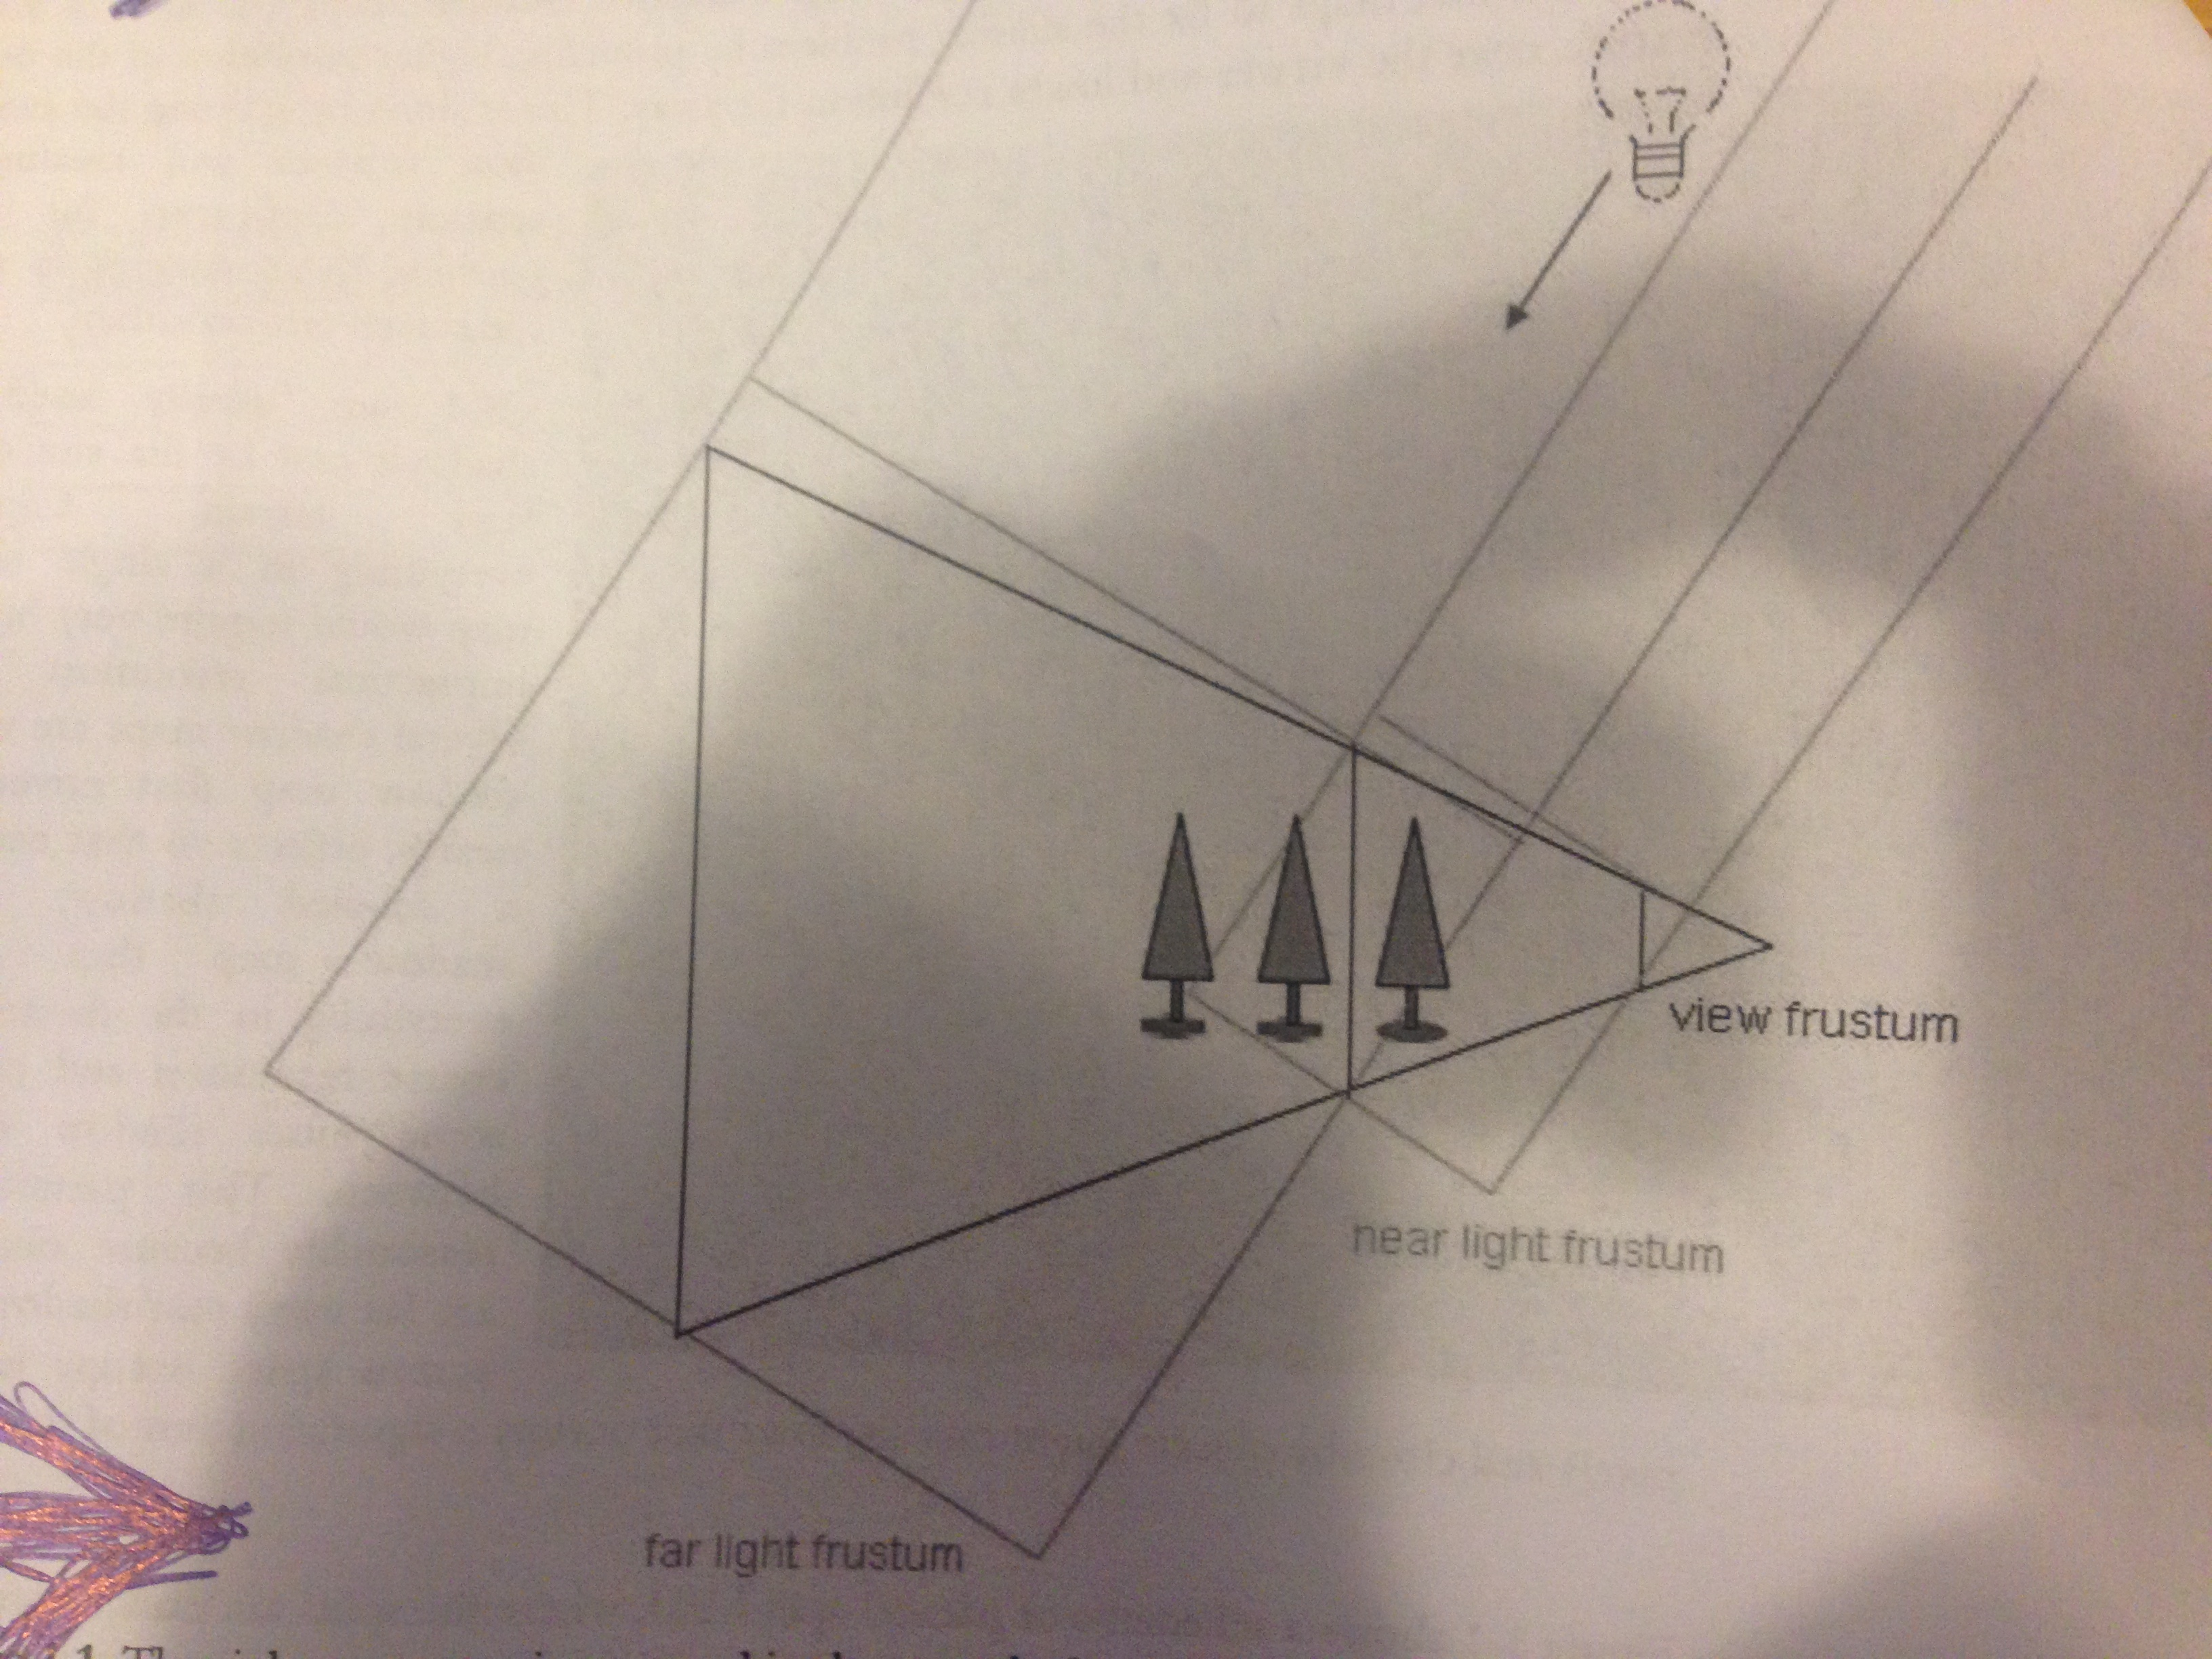
\includegraphics[width=140mm]{img/CSSHMAP1.JPG}
\caption{Opdelingen af view fustrums. Billedet fra \cite{CSM}}
\label{shadowmapdesc}
\end{figure}

Fordele
\begin{itemize}
  \item Funger godt for store scenen hvor lyskilden er solen.
  \item Shadow mappet skal generes hver gang kameraet flyttes. Dette bevirker at algoritmen kræver en del mere arbejde en shadow mapping
\end{itemize}

Ulemper:
\begin{itemize}
  \item Shadow mappet skal generes hver gang kameraet flyttes. Dette bevirker at algoritmen kræver en del mere arbejde en shadow mapping
  \item Skal opstilles og udregnes flere shadows maps hver gang.
\end{itemize}

\subsection{Diskussion af shadow mapping algoritmer}

Dette afsnittet vil diskuttere de tre algoritmer på generalle fordele og ulemper,  samt i forhold til hvad denne opgave ønsker at opnå dem skyggerne.

Da denne opgave kun vil arbejde men forholdsvis små og tildels afgrænsede scener vil Cascaded shadow maps blive sorteret fra. Cascaded shadow maps fungere rigtig godt for store scene, selv om det også ville kunne bruges med gode resultater på små scener ville dette være ekstra arbejde uden noget mærkbart bedre resultat. 

Perspective Shadow maps er på mange måde en god løsning fordi den ligger præcitationen hvor der er behov for den nemlig tæt på øjet. Det store problem med at objekter der ligger bag kameraet ikke kaster skygge skal der tages hånd om før algoritmen giver et tilfredsstillende resultat. Dette er ikke så lige til og er grunden til at denne algoritme ikke vælges. Dette efterlader Shadow maps med PCF som er den algoritmen rapporten vil arbejde videre med og implementere. Algoritmen vælges fordi den er hurtigt og egner sig godt til real-time grafik samt at de fleste aliasing problemer forholdsvis nemt og billigt kan løses.




\section{Status}

På nuværende tidspunkt er programmering og af shadow maps med PCF færdig programmeret og teori afsnittet, jeg mangler dog at færdiggøre test afsnittet i rapporten. Efter dette kigges på Shadow volumes der er sidste del af opgaven. Dette betyder dog at jeg er ca en 1 1/2 uge efter tidsplanen men regner med at jeg kan indhente dette og har derfor herunder lavet en opdateret tidsplan.
 
\begin{figure}[ht!]
\centering
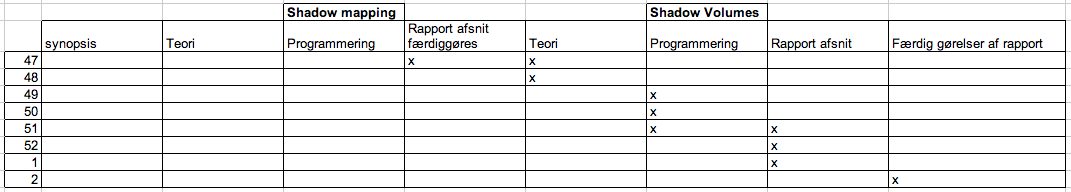
\includegraphics[width=140mm]{img/TIDSPLAN.PNG}
\caption{Opdateret tidsplan.}
\label{shadowmapdesc}
\end{figure}



\newpage 

\section{Litteratur}

\begin{thebibliography}{100} % 100 is a random guess of the total number of 
%references 
 
\addtolength{\leftmargin}{0.2in} % sets up alignment with the following line. 
\setlength{\itemindent}{-0.2in} 

\bibitem[RSC84]{PCF} 
 Rendering Antialiased Shadows with Depth Maps.
  William T. Reeves , David H. Salesin, Robert L. Cook 
  \emph{Computer Graphics, Volume 21}, 283-291, 1987.
  
  \bibitem[LW78]{SMAP} 
 CASTING CURVED SHADOWS ON CURVED SURFACES.
   Lance Williams
  \emph{Computer Graphics Lab New York Institute of Technology }, 1978.

  \bibitem[PSM02]{PSMAP} 
 Perspective Shadow Maps. 
  Marc Stamminger og George Drettakis.
  \emph{REVES - INRIA Sophia-Antipolis, France}, 2002.

  \bibitem[OGRED13]{PSMAP} 
 OpenGL Programming Guide.
  Dave Shreiner, Graham Sellers, John Kessenich og Bill Licea-Kane.
  \emph{The Khronos OpenGL ARB Working Group}, 2013.
        
    \bibitem[CSM07]{CSM} 
   Cascaded Shadow Maps
  Rouslan Dimitrov.
  \emph{NVIDIA Corporation}, 2007.
        
  
\end{thebibliography} 


\end{document}